\chapter*{Aufgabe 1}
\section*{a}
Die Methode gibt die Anzahl negativer Elemente plus der Elemente die mit v übereinstimmen, falls diese nicht negativ sind zurück. Falls ein Element von a[] am 2.,3.,oder 4. Bit eine 1 hat wird eine IllegalArgumentException geworfen.

\section*{b}
\begin{figure}[h]
	\centering
	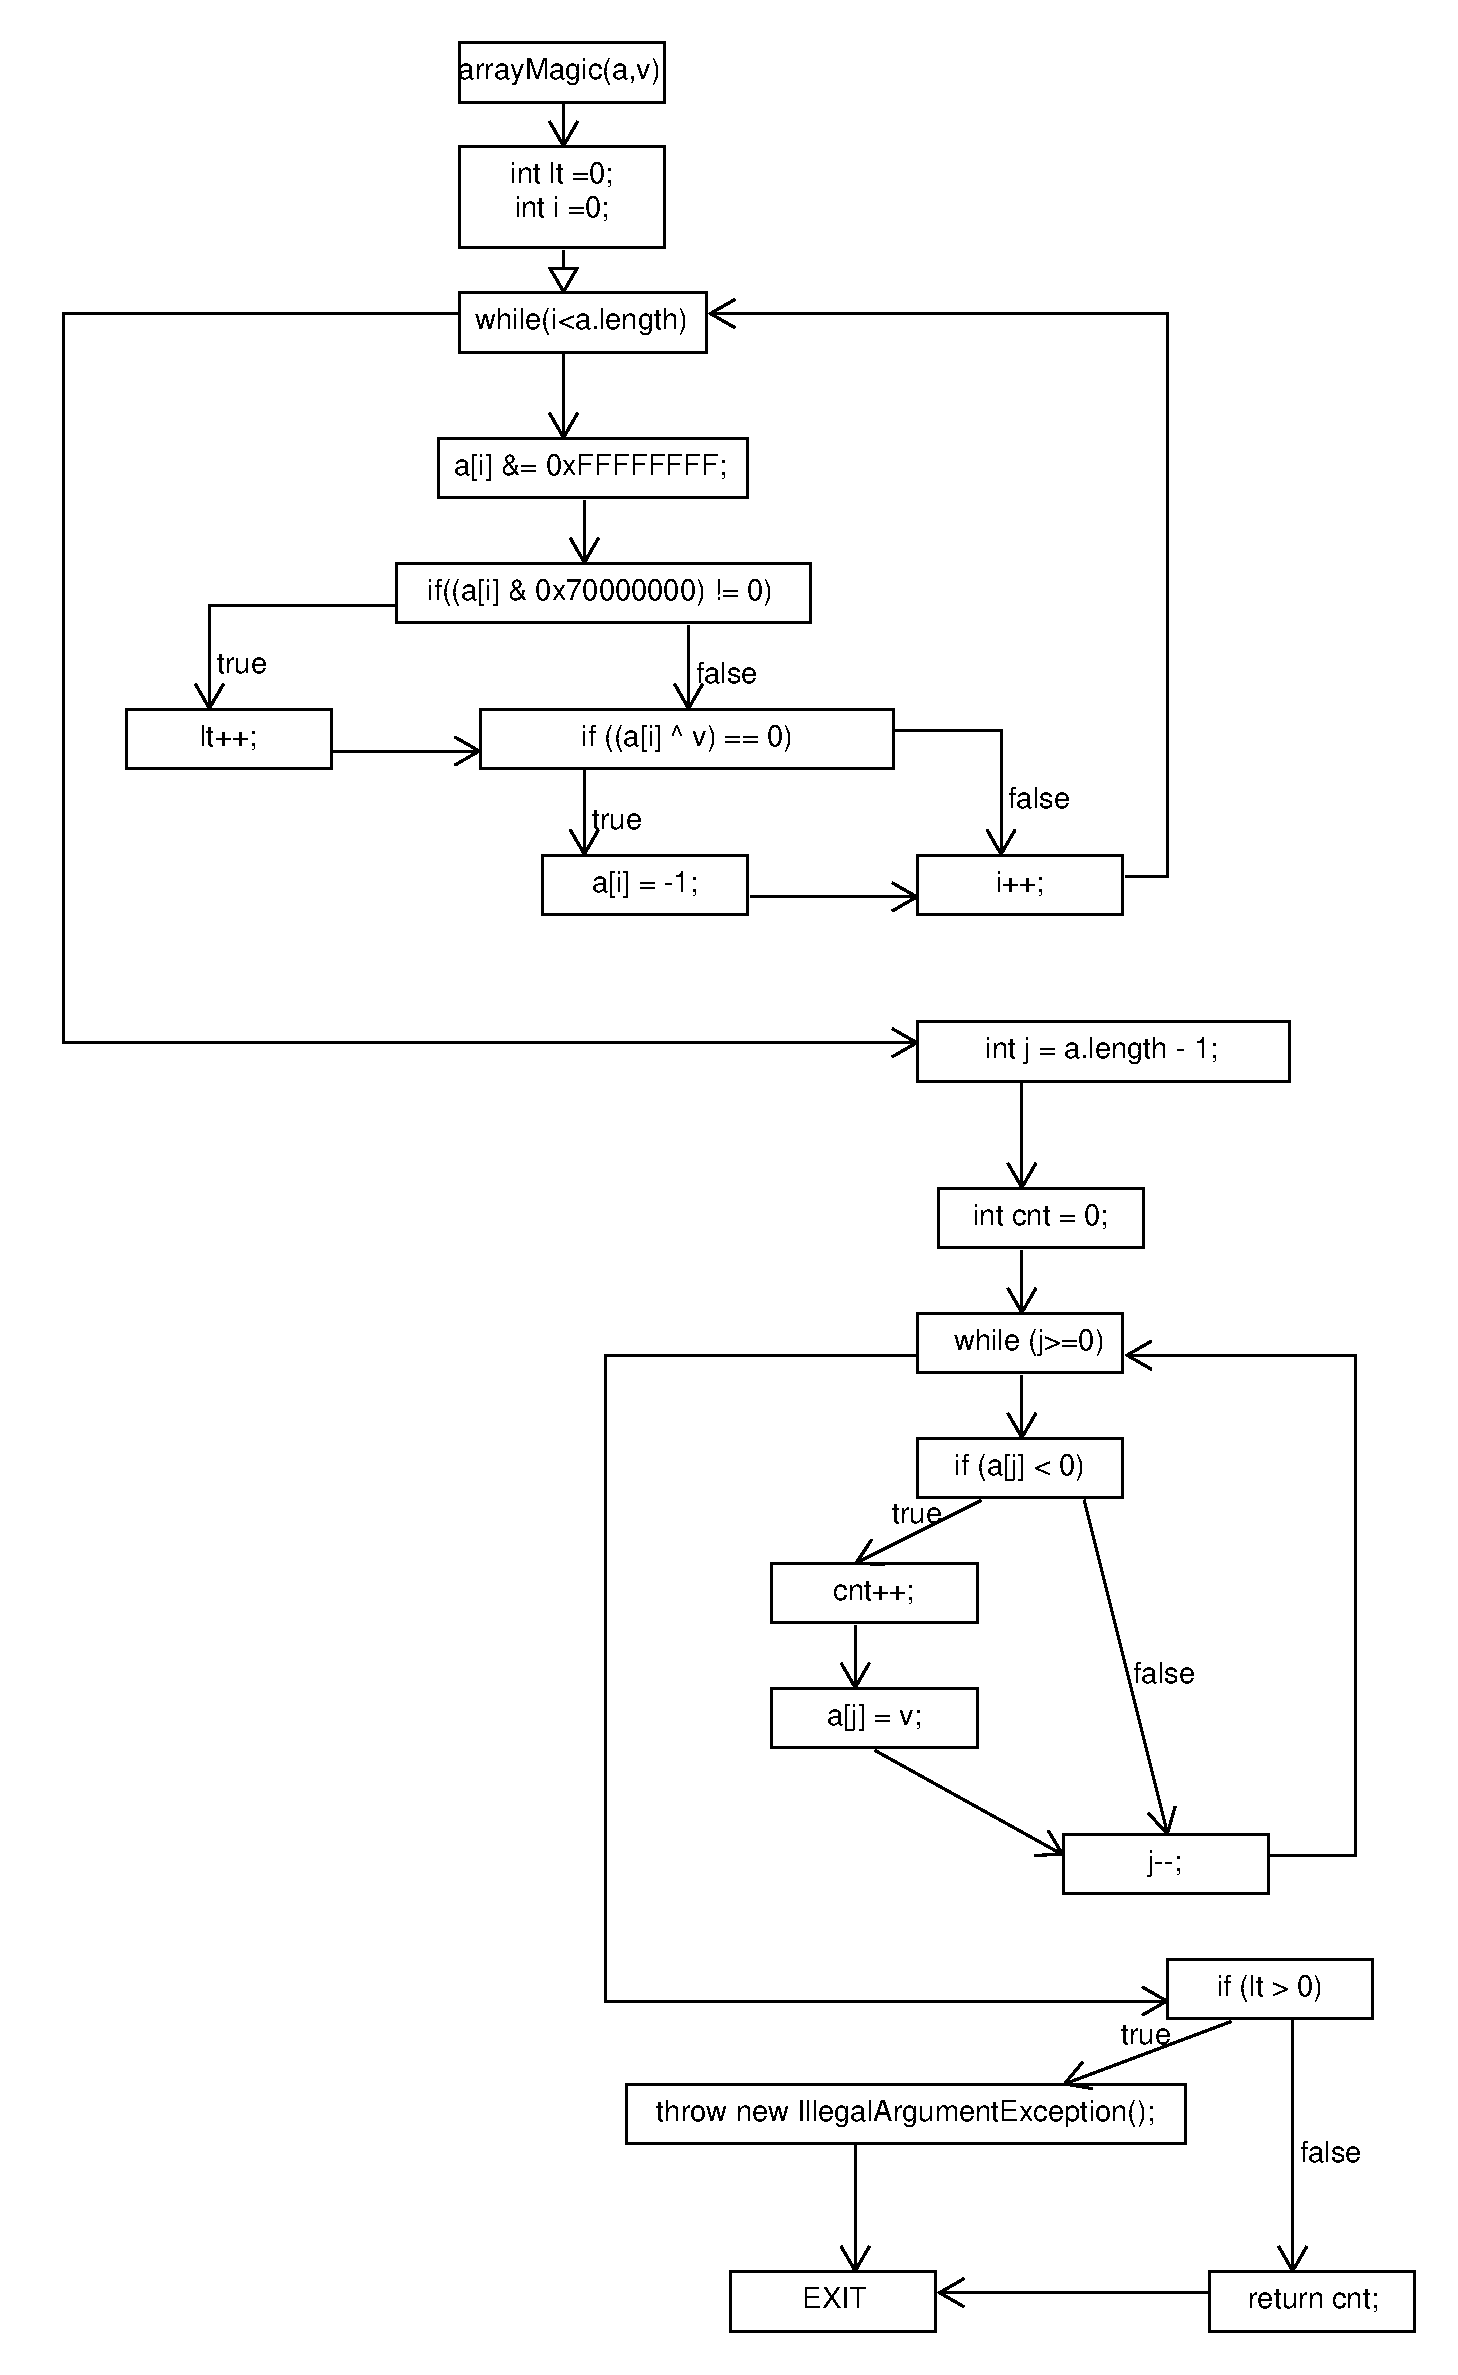
\includegraphics[width=0.8\textwidth, clip]{FlowChart.pdf}
	\caption{Kontrollflussgrpahe}
	\label{fig:flowChart}
\end{figure}
\section*{c}
Für die zyklomatische Komplexität nach der Formel $ C=E-N+2P$ ergibt sich mit den Werten
\begin{equation}
	C= 25-20+2 \doteq 1 = 7:
\end{equation}
Für einen Code mit einer so simplen Aufgabe ist die Komplexität schon sehr hoch.



Kanten:25
Knoten:20
P:2*1

C = E-n+ 2P

\section*{d}
Die Zeile 7 erfüllt keinen Zweck. Denn werden alle 32 Bits eines Integesrs mit 32 mal einer 1 Bitweise Undverknüpft, so erhält man wieder den selben Integer.
Die Zeile hat keinen Einfluss auf die Zyklische Komplexität, da ein Knoten und eine Kante dem Graphen hinzugefügt wird und sich so die Komplexität C nicht ändert.